\let\negmedspace\undefined
\let\negthickspace\undefined
\documentclass[journal]{IEEEtran}
\usepackage[a5paper, margin=10mm, onecolumn]{geometry}
\usepackage{lmodern} % Ensure lmodern is loaded for pdflatex
\usepackage{tfrupee} % Include tfrupee package

\setlength{\headheight}{1cm} % Set the height of the header box
\setlength{\headsep}{0mm}  % Set the distance between the header box and the top of the text

\usepackage{csquotes}
\usepackage{gvv-book}
\usepackage{gvv}
\usepackage{circuitikz}
\usepackage{cite}
\usepackage{amsmath,amssymb,amsfonts,amsthm}
\usepackage{algorithmic}
\usepackage{graphicx}
\usepackage{textcomp}
\usepackage{xcolor}
\usepackage{txfonts}
\usepackage{listings}
\usepackage{enumitem}
\usepackage{mathtools}
\usepackage{gensymb}
\usepackage{comment}
\usepackage[breaklinks=true]{hyperref}
\usepackage{tkz-euclide} 
\usepackage{listings}
% \usepackage{gvv}                                        
\def\inputGnumericTable{}                                 
\usepackage[latin1]{inputenc}                                
\usepackage{color}                                            
\usepackage{array}                                            
\usepackage{longtable}                                       
\usepackage{calc}                                             
\usepackage{multirow}                                         
\usepackage{hhline}                                           
\usepackage{ifthen}                                           
\usepackage{lscape}
\usepackage{caption}
\usepackage{tikz}
\usetikzlibrary{patterns}
\begin{document}

\bibliographystyle{IEEEtran}

\title{GATE 2016 CIVIL ENGINEERING}
\author{EE25BTECH11013 - Bhargav}
\maketitle
% \maketitle
% \newpage
% \bigskip
{\let\newpage\relax\maketitle}

\renewcommand{\thefigure}{\theenumi}
\renewcommand{\thetable}{\theenumi}
\setlength{\intextsep}{10pt} % Space between text and floats






\begin{enumerate}
\item Out of the following four sentences, select the most suitable sentence with respect to grammar and usage. \hfill \brak{GATE \ CE \ 2016}
\begin{enumerate}

\item I will not leave the place until the minister does not meet me.
\item I will not leave the place until the minister doesn't meet me.
\item I will not leave the place until the minister meet me.
\item I will not leave the place until the minister meets me.

\end{enumerate}

\item A rewording of something written or spoken is a  \hfill \brak{GATE \ CE \ 2016}
\begin{enumerate}
\begin{multicols}{2}
\item paraphrase
\item paradox
\item paradigm
\item paraffin
\end{multicols}
\end{enumerate}

\item Archimedes said, ``Give me a lever long enough and a fulcrum on which to place it, and I will move the world.'' The sentence above is an example of a \_\_\_\_\_\_ statement. \hfill \brak{GATE \ CE \ 2016}
\begin{enumerate}
\begin{multicols}{2}
\item figurative
\item collateral
\item literal
\item figurine
\end{multicols}
\end{enumerate}

\item If "relftaga" means carefree, "otaga" means careful and "fertaga" means careless, which of the following could mean "aftercare"? \hfill \brak{GATE \ CE \ 2016}
\begin{enumerate}
\begin{multicols}{2}
\item zentaga
\item tagafer
\item tagazen
\item relffer
\end{multicols}
\end{enumerate}

\item A cube is built using 64 cubic blocks of side one unit. After it is built, one cubic block is removed from every corner of the cube. The resulting surface area of the body (in square units) after the removal is . \hfill \brak{GATE \ GA \ 2016}
\begin{enumerate}
\begin{multicols}{2}
\item 56
\item 64
\item 72
\item 96
\end{multicols}
\end{enumerate}

\item A shaving set company sells 4 different types of razors: Elegance (Rs. 48), Smooth (Rs. 63), Soft (Rs. 78) and Executive (Rs. 173). The table below shows number of each razor sold in each quarter of a year. Which product contributes the greatest fraction to the annual revenue? \hfill \brak{GATE \ CE \ 2016}
\begin{enumerate}
\begin{multicols}{2}
\item Elegance 
\item Executive
\item Smooth
\item Soft
\end{multicols}
\end{enumerate}

\item Indian currency notes show denomination in at least 17 languages. This is evidence of \_\_\_\_\_\_. \hfill \brak{GATE \ CE \ 2016}
\begin{enumerate}
\begin{multicols}{2}
\item India is a country of exactly 17 languages.
\item Linguistic pluralism is the only indicator of diversity.
\item Indian currency notes have space for all languages.
\item Linguistic pluralism is strong evidence of India's diversity.
\end{multicols}
\end{enumerate}

\item Four players $P, Q, R, S$ have the following relations: $P$ always beats $Q$; $R$ always beats $S$; $S$ loses to $P$ only sometimes; $R$ always loses to $Q$. Which of the following is correct? \hfill \brak{GATE \ CE \ 2016}
\begin{enumerate}
\begin{multicols}{2}
\item (i) only
\item (ii) only
\item (i) and (ii)
\item neither (i) nor (ii)
\end{multicols}
\end{enumerate}

\item If $f(x) = 2x^7 + 3x^{-5}$, which of the following is a factor of $f(x)$? \hfill \brak{GATE \ CE \ 2016}
\begin{enumerate}
\begin{multicols}{2}
\item $(x^3+8)$
\item $(x-1)$
\item $(2x-5)$
\item $(x+1)$
\end{multicols}
\end{enumerate}

\item In a process, the number of cycles to failure decreases exponentially with load. At $80$ units load, failure in 100 cycles; at half load, failure in 10000 cycles. Find the load for failure in 5000 cycles. \hfill \brak{GATE \ CE \ 2016}
\begin{enumerate}
\begin{multicols}{2}
\item 40.00
\item 46.02
\item 60.01
\item 92.02
\end{multicols}
\end{enumerate}
\end{enumerate}

\subsection*{Civil Engineering - Set 1}

\begin{enumerate}[resume]
\item Newton-Raphson method is used for root of $3x - e^x + \sin x = 0$ with initial trial $x_0 = 0.333$. Find the next approximation (3 decimal places). \hfill \brak{GATE \ CE \ 2016} \\[0.5em]
\textbf{Answer:} \_\_\_\_\_

\item The type of PDE
\begin{align}
\frac{\partial^2 P}{\partial x^2} + \frac{\partial^2 P}{\partial y^2} + 3\frac{\partial^2 P}{\partial x \partial t} + 2\frac{\partial P}{\partial x} - \frac{\partial P}{\partial t} = 0
\end{align}
is \hfill \brak{GATE \ CE \ 2016}
\begin{enumerate}
\begin{multicols}{2}
\item elliptic
\item parabolic
\item hyperbolic
\item none of these
\end{multicols}
\end{enumerate}

\item If the entries in each column of a square matrix $M$ add up to $1$, then an eigenvalue is \hfill \brak{GATE \ CE \ 2016}
\begin{enumerate}
\begin{multicols}{2}
\item 4
\item 3
\item 2
\item 1
\end{multicols}
\end{enumerate}

\item Type II error in hypothesis testing is \hfill \brak{GATE \ CE \ 2016}
\begin{enumerate}
\begin{multicols}{2}
\item Accept $H_0$ when it is false
\item Reject $H_0$ when it is true
\item Reject $H_0$ when it is false
\item Accept $H_0$ when it is true
\end{multicols}
\end{enumerate}

\item The solution of
\begin{align}
\frac{\partial^2 u}{\partial t^2} = \alpha^2 \frac{\partial^2 u}{\partial x^2}
\end{align}
is of the form: \hfill \brak{GATE \ CE \ 2016}
\begin{enumerate}
\begin{multicols}{2}
\item $\left(C_1 e^{kx} + C_2 e^{-kx}\right)\cos(\alpha kt)$
\item $\left(C_1 e^{kx} + C_2 e^{-kx}\right)Ce^{\alpha kt}$
\item $\left(C_1 \cos kx + C_2 \sin kx\right)e^{\alpha kt}$
\item $\left(C_1 \cos kx + C_2 \sin kx\right)\sin(\alpha kt)$
\end{multicols}
\end{enumerate}
\maketitle

\item Consider the plane truss with load $P$ as shown in the figure. Let the horizontal and vertical reactions at the joint B be $H_B$ and $V_B$, respectively and $V_C$ be the vertical reaction at the joint C.

\begin{figure}[H]
    \centering
    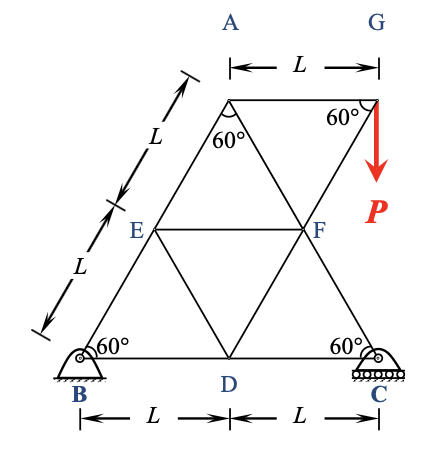
\includegraphics[width=0.6\columnwidth]{figs/Q16.png} 
    \caption{}
    \label{fig:placeholder}
\end{figure}

Which one of the following sets gives the correct values of $V_B$, $H_B$ and $V_C$? \hfill \brak{GATE \ CE \ 2016}
\begin{enumerate}
\begin{multicols}{2}
\item $V_B = 0, \ H_B = 0, \ V_C = P$
\item $V_B = P\sqrt{2}, \ H_B = 0, \ V_C = -P/2$
\item $V_B = P/2, \ H_B = P\sin 60^\degree, \ V_C = P/2$
\item $V_B = P/2, \ H_B = P\cos 60^\degree, \ V_C = 0$
\end{multicols}
\end{enumerate}


\item In shear design of an RC beam, other than the allowable shear strength of concrete $(\tau_c)$, there is also an additional check suggested in IS 456-2000 with respect to the maximum permissible shear stress $(\tau_{c \ \text{max}})$. The check for $\tau_{c \ \text{max}}$ is required to take care of \hfill \brak{GATE \ CE \ 2016}
\begin{enumerate}
\begin{multicols}{2}
\item Additional shear resistance from reinforcing steel
\item Additional shear resistance from strain hardening
\item Possibility of failure of concrete by diagonal tension
\item Possibility of crushing of concrete by diagonal compression
\end{multicols}
\end{enumerate}


\item The semi-compact section of a laterally unsupported steel beam has an elastic section modulus, plastic section modulus and design bending compressive stress of $550 \ mm^3$, $650 \ mm^3$ and $200 \ MPa$, respectively. The shape factor (plastic/elastic) expressed in terms of the section is \hfill \brak{GATE \ CE \ 2016}
\begin{enumerate}
\begin{multicols}{2}
\item 0.85
\item 1.18
\item 1.33
\item 1.41
\end{multicols}
\end{enumerate}


\item Bull's trench kiln is used in the manufacturing of \hfill \brak{GATE \ CE \ 2016}
\begin{enumerate}
\begin{multicols}{2}
\item lime
\item cement
\item bricks
\item none of these
\end{multicols}
\end{enumerate}


\item The compound which is largely responsible for initial setting and early strength gain of Ordinary Portland Cement is \hfill \brak{GATE \ CE \ 2016}
\begin{enumerate}
\begin{multicols}{2}
\item $C_3A$
\item $C_3S$
\item $C_2S$
\item $C_4AF$
\end{multicols}
\end{enumerate}


\item In the consolidated undrained triaxial test on a saturated soil sample, the pore water pressure is zero  \hfill \brak{GATE \ CE \ 2016}
\begin{enumerate}
    \item during shearing stage only
    \item at the end of consolidation stage only
    \item both at the end of consolidation and during shearing stages
    \item under none of the above conditions
\end{enumerate}


\item A fine grained soil is found to be plastic in the water content range of 26 -- 48\%. As per Indian Standard Classification System, the soil is classified as \hfill \brak{GATE \ CE \ 2016}
\begin{enumerate}
\begin{multicols}{2}
\item CL
\item CH
\item CL-ML
\item CI
\end{multicols}
\end{enumerate}

\item A vertical cut is to be made in a soil mass having cohesion \( c \), angle of internal friction \( \varphi \), and unit weight \( \gamma \). Considering \( K_a \) and \( K_p \) as the coefficients of active and passive earth pressures, respectively, the maximum depth of unsupported excavation is \hfill \brak{GATE \ CE \ 2016}
\begin{enumerate}
\begin{multicols}{2}
\item \( \frac{4c}{\gamma \sqrt{K_p}} \)
\item \( \frac{2c \sqrt{K_p}}{\gamma} \)
\item \( \frac{4c \sqrt{K_a}}{\gamma} \)
\item \( \frac{4c}{\gamma \sqrt{K_a}} \)
\end{multicols}
\end{enumerate}

\item The direct runoff hydrograph in response to 5 cm rainfall excess in a catchment is shown in the figure. The area of the catchment (expressed in hectares) is \rule{3cm}{0.15mm} \hfill \brak{GATE \ CE \ 2016}

\begin{figure}[H]
    \centering
    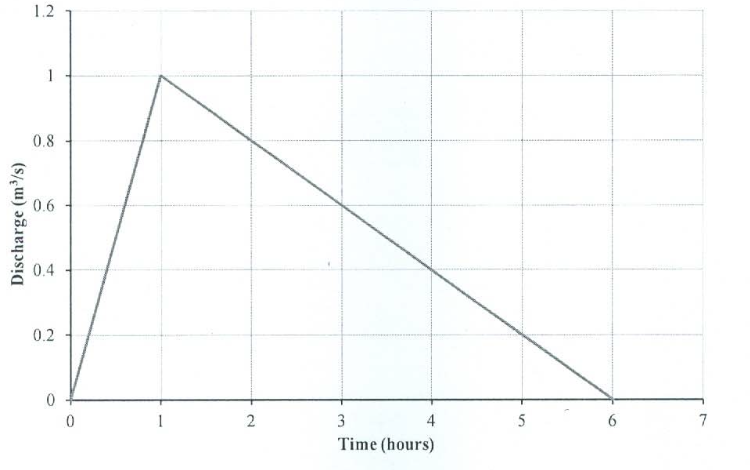
\includegraphics[width=0.6\columnwidth]{figs/Q24.png} 
    \caption{}
    \label{fig:placeholder}
\end{figure}

\item The types of flood routing (Group-I) and the appropriate used for its purpose (Group-II) are given below: \hfill \brak{GATE \ CE \ 2016}
\begin{enumerate}
\item[(P)] Storage Indication Method \hfill 1. Reservoir situation
\item[(Q)] Muskingum Method \hfill 2. Open channel routing
\item[(R)] Unit Hydrograph \hfill 3. Surface runoff estimation
\item[(S)] Hydrological routing \hfill 4. Groundwater movement
\end{enumerate}
The correct combination is
\begin{enumerate}
\begin{multicols}{2}
\item P-1, Q-2, R-3, S-4
\item P-2, Q-1, R-3, S-4
\item P-3, Q-4, R-1, S-2
\item P-4, Q-1, R-2, S-3
\end{multicols}
\end{enumerate}

\item The pre-jump Froude Number for a particular flow in a horizontal rectangular channel is $10$. The ratio of sequent depths \brak{i.e. \ post-jump \ depth \ to \ pre-jump \ depth} is \hfill \brak{GATE \ CE \ 2016}

\item Pre-cursors to photochemical oxidants are \hfill \brak{GATE \ CE \ 2016}
\begin{enumerate}
\begin{multicols}{2}
\item NOx, VOCs and sunlight
\item SO$_2$, CO and sunlight
\item CO, NOx and sunlight
\item SO$_2$, NH$_3$ and sunlight
\end{multicols}
\end{enumerate}


\item Crown corrosion in a reinforced concrete sewer is caused by: \hfill \brak{GATE \ CE \ 2016}
\begin{enumerate}
\begin{multicols}{2}
\item H$_2$S
\item CO$_2$
\item CH$_4$
\item NH$_3$
\end{multicols}
\end{enumerate}


\item It was decided to construct a fabric filter, using bags of $0.45$ m diameter and $7.5$ m long, for removing industrial stack gas containing particulates. The expected rate of airflow into the filter is $10$ m$^3$/s. If the filtering velocity is $2.0$ m/min, the minimum number of bags \brak{rounded \ to \ nearest \
higher \ integer} required for continuous cleaning operation is \hfill \brak{GATE \ CE \ 2016}
\begin{enumerate}
\begin{multicols}{2}
\item $27$
\item $29$
\item $31$
\item $32$
\end{multicols}
\end{enumerate}


\item Match the items in Group -- I with those in Group -- II and choose the right combination. \hfill \brak{GATE \ CE \ 2016}
\begin{enumerate}
\item[(P)] Aerated lagoon \hfill 1. Group -- III
\item[(Q)] Activated sludge process \hfill 2. Microstraining
\item[(R)] Coagulation \hfill 3. Autotrophic bacteria
\item[(S)] Nitrification \hfill 4. Heterotrophic bacteria
\end{enumerate}
\begin{enumerate}
\begin{multicols}{2}
\item P-3, Q-4, R-2, S-1
\item P-2, Q-1, R-3, S-4
\item P-4, Q-3, R-2, S-1
\item P-1, Q-4, R-3, S-2
\end{multicols}
\end{enumerate}

\item During a forensic investigation of pavement failure, an engineer reconstructed the graphs P, Q, R and S, using partial and damaged old reports. \hfill \brak{GATE \ CE \ 2016}

\begin{figure}[H]
    \centering
    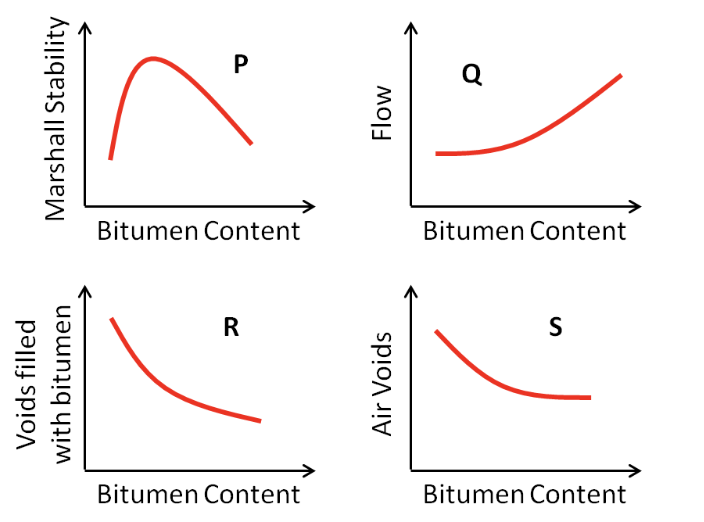
\includegraphics[width=0.6\columnwidth]{figs/Q31.png} 
    \caption{}
    \label{fig:placeholder}
\end{figure}

\begin{enumerate}
\begin{multicols}{2}
\item P, Q, R
\item P, Q, S
\item Q, R, S
\item P, S, R
\end{multicols}
\end{enumerate}

\item In a one-lane one-way homogeneous traffic stream, the observed average headway is $3.0 \ s$. The flow (expressed in vehicles/hr) in this traffic stream is \hfill \brak{GATE \ CE \ 2016}
\begin{enumerate}
\begin{multicols}{2}
\item 1200
\item 900
\item 720
\item 600
\end{multicols}
\end{enumerate}

\item The minimum number of satellites needed for a GPS to determine its position precisely is \hfill \brak{GATE \ CE \ 2016}
\begin{enumerate}
\begin{multicols}{2}
\item 2
\item 3
\item 4
\item 24
\end{multicols}
\end{enumerate}

\item The system that uses the Sun as a source of electromagnetic energy and records the naturally radiated and reflected energy from the object is called \hfill \brak{GATE \ CE \ 2016}
\begin{enumerate}
\begin{multicols}{2}
\item Geographical Information System
\item Global Positioning System
\item Passive Remote Sensing
\item Active Remote Sensing
\end{multicols}
\end{enumerate}

\item The staff reading taken on a workshop floor using a level is $0.645 \ m$. The inverted staff reading taken to the bottom of a beam is $2.950 \ m$. The reduced level of the floor is $40.500 \ m$. The reduced level (expressed in m) of the bottom of the beam is \hfill \brak{GATE \ CE \ 2016}
\begin{enumerate}
\begin{multicols}{2}
\item 44.105
\item 43.460
\item 42.815
\item 41.145
\end{multicols}
\end{enumerate}

\item Probability density function of a random variable $X$ is given below:
\begin{align}
f(x) = \begin{cases}
0.25 & \text{if } 1 \leq x \leq 5 \\
0 & \text{otherwise}
\end{cases}
\end{align}
P(X $>$ 4) is \hfill \brak{GATE \ CE \ 2016}
\begin{enumerate}
\begin{multicols}{2}
\item $\frac{3}{4}$
\item $\frac{2}{4}$
\item $\frac{1}{4}$
\item $\frac{1}{2}$
\end{multicols}
\end{enumerate}

\item The value of 
\begin{align}
\int_{0}^{\pi/3} \frac{1}{1+3\tan^2x} dx + \int_{0}^{\pi/3} \frac{\sin x}{x} dx
\end{align}
is \hfill \brak{GATE \ CE \ 2016}
\begin{enumerate}
\begin{multicols}{2}
\item $\frac{\pi}{6}$
\item $\frac{\pi}{3}$
\item $\frac{\pi}{2}$
\item 1
\end{multicols}
\end{enumerate}

\item The area of the region bounded by the parabola $y = x^2 + 1$ and the straight line $x + y = 3$ is \hfill \brak{GATE \ CE \ 2016}
\begin{enumerate}
\begin{multicols}{2}
\item $\frac{59}{6}$
\item $\frac{9}{2}$
\item $\frac{10}{3}$
\item $\frac{7}{6}$
\end{multicols}
\end{enumerate}

\item The magnitudes of vectors P, Q and R are 100 kN, 250 kN and 150 kN, respectively. The respective values of the magnitude (in kN) and the direction (with respect to the x-axis) of the resultant vector are \hfill \brak{GATE \ CE \ 2016}

\begin{figure}[H]
    \centering
    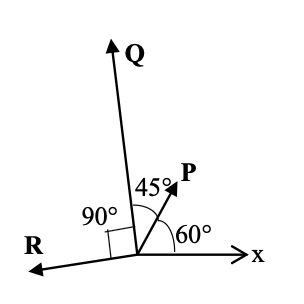
\includegraphics[width=0.6\columnwidth]{figs/Q39.png} 
    \caption{}
    \label{fig:placeholder}
\end{figure}

\begin{enumerate}
\begin{multicols}{2}
\item 299.90 and 96.0$^\degree$
\item 368.1 and 94.7$^\degree$
\item 330.4 and 118.9$^\degree$
\item 400.1 and 113.5$^\degree$
\end{multicols}
\end{enumerate}

\item The respective expressions for complimentary function and particular integral part of the solution of the differential equation $\frac{d^2x}{dt^2} + 3\frac{dx}{dt} + 12x = 108t^2$ are \hfill \brak{GATE \ CE \ 2016}
\begin{enumerate}
\item $[c_1 + c_2 t + \sin \sqrt{3}t + c_3 \cos \sqrt{3}t]$ and $[3t^2 - 12t^2 + c]$
\item $[x + c_1 \sin \sqrt{3}t + c_2 \cos \sqrt{3}t]$ and $[5t^2 - 12t^2 + c]$
\item $[c_1 t + c_2 \sin \sqrt{3}t + c_3 \cos \sqrt{3}t]$ and $[5t^2 - 12t^2 + c]$
\item $[c_1 + c_2 t + \sin \sqrt{3}t + c_3 \cos \sqrt{3}t]$ and $[5t^2 - 12t^2 + c]$
\end{enumerate}

\item A 3 m long simply supported beam of uniform cross section is subjected to a uniformly distributed load of $w = 20 \ \text{kN/m}$ in the central 1 m as shown. If the flexural rigidity (EI) of the beam is $30 \times 10^6 \ \text{Nm}^2$, the maximum slope (expressed in radians) of the deformed beam is \hfill \brak{GATE \ CE \ 2016}

\begin{figure}[H]
    \centering
    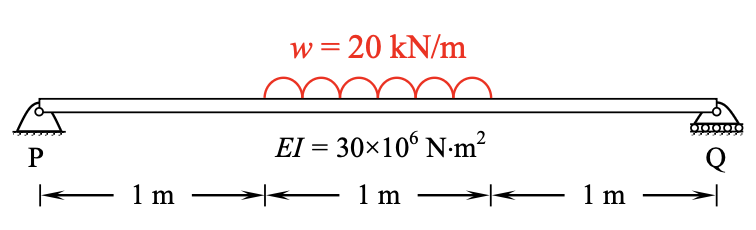
\includegraphics[width=0.3\columnwidth]{figs/Q41.png} 
    \caption{}
    \label{fig:placeholder}
\end{figure}

\begin{enumerate}
\begin{multicols}{2}
\item $0.681 \times 10^{-3}$
\item $0.943 \times 10^{-3}$
\item $4.310 \times 10^{-3}$
\item $5.910 \times 10^{-3}$
\end{multicols}
\end{enumerate}

\item Two beams PQ (fixed at P and with a roller support at Q, as shown in Figure I, which allows vertical movement) and XZ (with a hinge at Y) are shown in the Figures I and II respectively. The spans of PQ and XZ are $L$ and $2L$ respectively. Both the beams are under the action of uniformly distributed load $(w)$ and have the same flexural stiffness, $EI$ (where, $E$ and $I$ respectively denote modulus of elasticity and moment of inertia about axis of bending). Let the maximum deflection and maximum rotation be $\delta_{max1}$ and $\theta_{max1}$ respectively, in the case of beam PQ and the corresponding quantities for the beam XZ be $\delta_{max2}$ and $\theta_{max2}$ respectively. \hfill \brak{GATE \ CE \ 2016}

\begin{figure}[H]
    \centering
    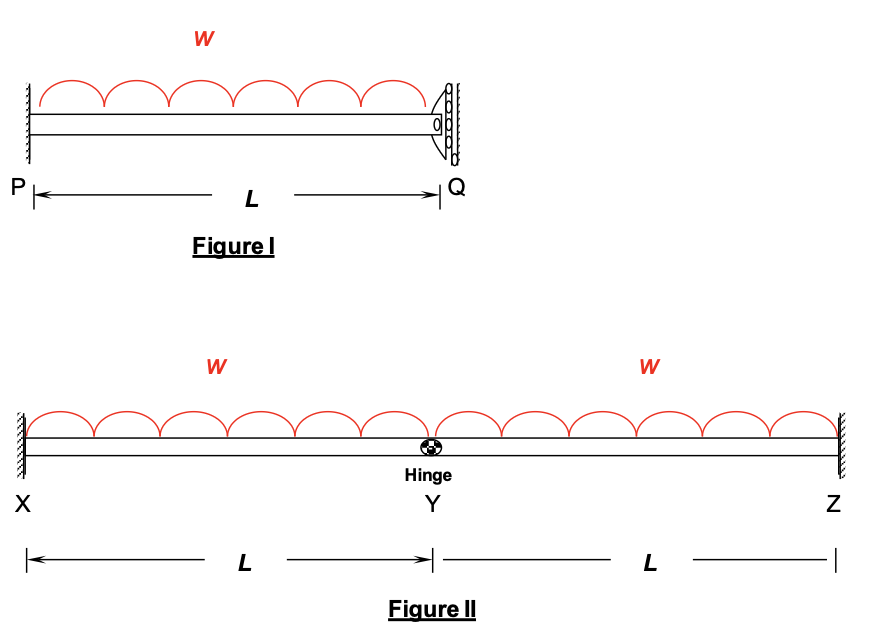
\includegraphics[width=0.3\columnwidth]{figs/Q42.png} 
    \caption{}
    \label{fig:placeholder}
\end{figure}

Which one of the following relationships is true?
\begin{enumerate}
\begin{multicols}{2}
\item $\delta_{max1} \neq \delta_{max2}$ and $\theta_{max1} \neq \theta_{max2}$
\item $\delta_{max1} = \delta_{max2}$ and $\theta_{max1} \neq \theta_{max2}$
\item $\delta_{max1} \neq \delta_{max2}$ and $\theta_{max1} = \theta_{max2}$
\item $\delta_{max1} = \delta_{max2}$ and $\theta_{max1} = \theta_{max2}$
\end{multicols}
\end{enumerate}

\item A plane truss with applied loads is shown in the figure. \hfill \brak{GATE \ CE \ 2016}

The members which do not carry any force are:

\begin{figure}[H]
    \centering
    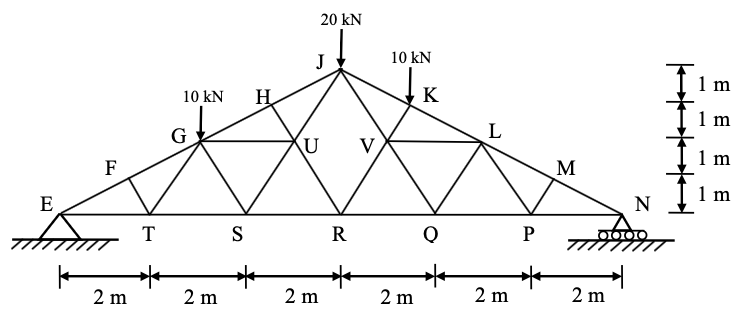
\includegraphics[width=0.3\columnwidth]{figs/Q43.png} 
    \caption{}
    \label{fig:placeholder}
\end{figure}

\begin{enumerate}
\begin{multicols}{2}
\item FT, TG, HU, MP, PL
\item ET, GS, UR, VR, QL
\item FT, GS, HU, MP, QL
\item MP, PL, HU, FT, UR
\end{multicols}
\end{enumerate}

\item A rigid member ACB is shown in the figure. The member is supported at A and B by pinned and guided roller supports, respectively. A force $P$ acts at C as shown. Let $R_{Ah}$ and $R_{Bh}$ be the horizontal reactions at supports A and B, respectively, and $R_{Av}$ be the vertical reaction at support A. Self-weight of the member may be ignored. \hfill \brak{GATE \ CE \ 2016}

\begin{figure}[H]
    \centering
    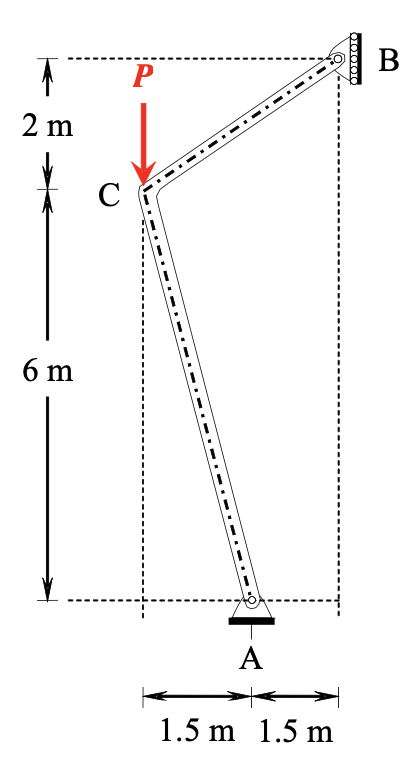
\includegraphics[width=0.6\columnwidth]{figs/Q44.png} 
    \caption{}
    \label{fig:placeholder}
\end{figure}

Which one of the following sets gives the correct magnitudes of $R_{Av}$, $R_{Ah}$ and $R_{Bh}$?
\begin{enumerate}
\begin{multicols}{2}
\item $R_{Av} = 0; \ R_{Bh} = \frac{1}{3}P; \ R_{Ah} = \frac{2}{3}P$
\item $R_{Av} = 0; \ R_{Bh} = \frac{2}{3}P; \ R_{Ah} = \frac{1}{3}P$
\item $R_{Av} = P; \ R_{Bh} = \frac{3}{8}P; \ R_{Ah} = \frac{1.5}{8}P$
\item $R_{Av} = P; \ R_{Bh} = \frac{1.5}{8}P; \ R_{Ah} = \frac{1.5}{8}P$
\end{multicols}
\end{enumerate}

\item A reinforced concrete (RC) beam with width of $250 \ mm$ and effective depth of $400 \ mm$ is reinforced with Fe415 steel. As per the provisions of IS $456$ - $2000$, the minimum and maximum amount of tensile reinforcement (expressed in $mm^2$) for the section are, respectively: \hfill \brak{GATE \ CE \ 2016}
\begin{enumerate}
\begin{multicols}{2}
\item 250 and 3500
\item 205 and 4000
\item 270 and 2000
\item 300 and 2500
\end{multicols}
\end{enumerate}

\item For M25 concrete with creep coefficient of $1.5$, the long-term static modulus of elasticity (expressed in MPa) as per the provisions of IS:$456$ - $2000$ is  \hfill \brak{GATE \ CE \ 2016}

\item A propped cantilever of span $L$ carries a vertical concentrated load at the mid-span. If the plastic moment capacity of the section is $M_p$, the magnitude of the collapse load is   \hfill \brak{GATE \ CE \ 2016}
\begin{enumerate}
\begin{multicols}{4}
\item $\frac{8M_p}{L}$
\item $\frac{6M_p}{L}$
\item $\frac{4M_p}{L}$
\item $\frac{2M_p}{L}$
\end{multicols}
\end{enumerate}

\item Two plates are connected by fillet welds of size $10 \ mm$ and subjected to tension. The thickness of each plate is $12 \ mm$. The yield stress and the ultimate tensile stress of steel are $250 \ MPa$ and $410 \ MPa$, respectively. The welding is done in the workshop $(\gamma_{mw} = 1.25)$.  
As per the Limit State Method of IS 800: 2007, the minimum length (rounded off to the nearest higher multiple of $5 \ mm$) of each weld to transmit a force $P$ equal to $270 \ kN$ (factored) is  \hfill \brak{GATE \ CE \ 2016}

\begin{figure}[H]
    \centering
    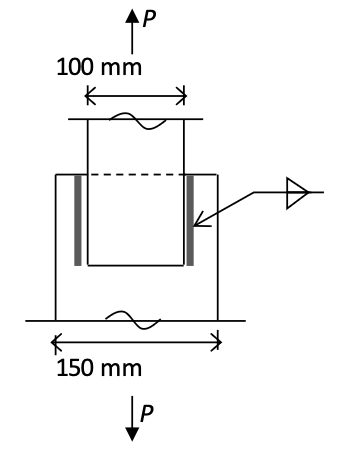
\includegraphics[width=0.6\columnwidth]{figs/Q48.png} 
    \caption{}
    \label{fig:placeholder}
\end{figure}

\begin{enumerate}
    \item $90 \ mm$
    \item $105 \ mm$
    \item $110 \ mm$
    \item $115 \ mm$
\end{enumerate}

\item The Optimistic Time (O), Most likely Time (M) and Pessimistic Time (P) (in days) of the activities in the critical path are given below in the format O-M-P:  

\begin{figure}[H]
    \centering
    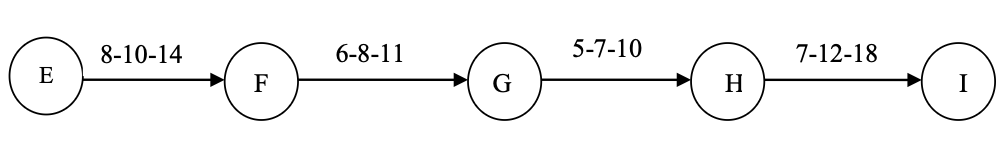
\includegraphics[width=0.6\columnwidth]{figs/Q49.png} 
    \caption{}
    \label{fig:placeholder}
\end{figure}

The expected completion time (in days) of the project is \_\_\_\_\_\_ \hfill \brak{GATE \ CE \ 2016}

\item The porosity $(n)$ and the degree of saturation $(S)$ of a soil sample are $0.7$ and $40\%$, respectively. In a $100 \ m^3$ volume of the soil, the volume (expressed in $m^3$) of air is \_\_\_\_\_\_ \hfill \brak{GATE \ CE \ 2016}

\item A homogeneous gravity retaining wall supporting a cohesionless backfill has a height of $6 \ m$ and base width $4 \ m$. The lateral active earth pressure at the bottom of the wall is $40 \ kPa$. The minimum weight of the wall \brak{expressed \ in \ kN \ per \ m \ length} required to prevent it from overturning about its toe \brak{Point \ P} is:  \hfill \brak{GATE \ CE \ 2016}

\begin{figure}[H]
    \centering
    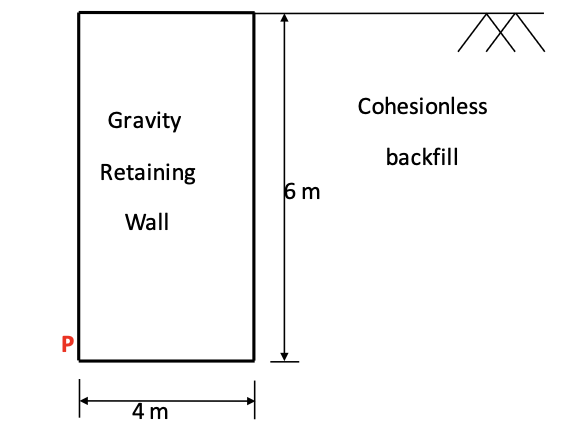
\includegraphics[width=0.6\columnwidth]{figs/Q51.png} 
    \caption{}
    \label{fig:placeholder}
\end{figure}
\begin{enumerate}
    \item 120
    \item 180
    \item 240
    \item 360
\end{enumerate}

\item An undisturbed soil sample was taken from the middle of a clay layer (i.e., $1.5 \ m$ below GL). The water table was at the top of clay layer. Laboratory test results are as follows:  \hfill \brak{GATE \ CE \ 2016}

\begin{center}
\begin{tabular}{ll}
    \textbf{Group I} & \textbf{Group II} \\
    P. Ferrite & 1. Hexagonal Close Packed (HCP) \\
    Q. Austenite & 2. Body Centered Cubic (BCC) \\
    R. Martensite & 3. Body Centered Tetragonal (BCT) \\
    & 4. Face Centered Cubic (FCC)
\end{tabular}
\end{center}

\begin{figure}[H]
    \centering
    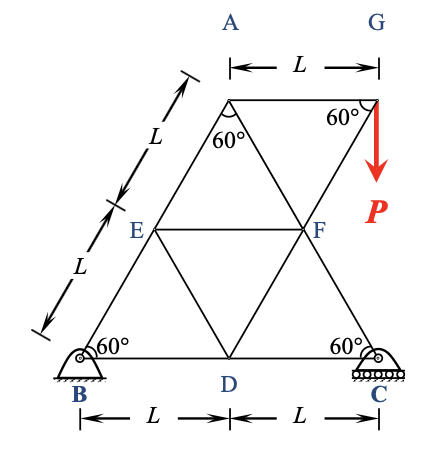
\includegraphics[width=0.6\columnwidth]{figs/Q16.png} 
    \caption{}
    \label{fig:placeholder}
\end{figure}

A compacted fill of $2.5 \ m$ height with unit weight of $20 \ kN/m^3$ is placed at the ground level.  

Assuming unit weight of water as $10 \ kN/m^3$, the ultimate consolidation settlement (expressed in mm) of the clay layer is \_\_\_\_\_\_

\item A seepage flow condition exists in a soil mass. The saturated unit weight of the soil $\gamma_{sat} = 18 \ \text{kN/m}^3$. Using unit weight of water $\gamma_w = 9.81 \ \text{kN/m}^3$, the effective vertical stress \brak{expressed \ in \ kN/m2} on plane $X$--$X$ is \_\_\_\_\_\_ \hfill \brak{GATE \ CE \ 2016}

\begin{figure}[H]
    \centering
    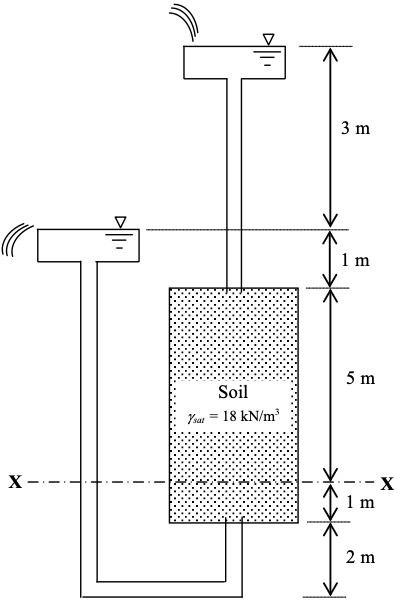
\includegraphics[width=0.6\columnwidth]{figs/Q53.png}
    \caption{}
    \label{fig:placeholder}
\end{figure}

\item A drained triaxial compression test on a saturated clay yielded the effective shear strength parameters as $c' = 15 \ kPa$ and $\phi' = 22^\degree$. Consolidated Undrained triaxial test on an identical sample of this clay at a cell pressure of $200 \ kPa$ developed a pore water pressure of $150 \ kPa$ at failure. The deviator stress (expressed in kPa) at failure is \_\_\_\_\_\_ \hfill \brak{GATE \ CE \ 2016}

\item A concrete gravity dam section is shown. Assuming unit weight of water as $10 \ \text{kN/m}^3$ and unit weight of concrete as $24 \ \text{kN/m}^3$, the uplift force per unit length of the dam (expressed in kN/m) at $PQ$ is \_\_\_\_\_\_ \hfill \brak{GATE \ CE \ 2016}

\begin{figure}[H]
    \centering
    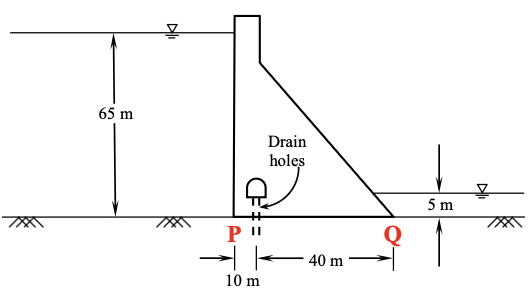
\includegraphics[width=0.6\columnwidth]{figs/Q55.png} 
    \caption{}
    \label{fig:placeholder}
\end{figure}

\item Seepage is occurring through a porous media. The hydraulic conductivity values $k_1, k_2, k_3$ are in m/day. The seepage discharge (m$^3$/day per m) through the porous media at section $PQ$ is  \hfill \brak{GATE \ CE \ 2016}

\begin{figure}[H]
    \centering
    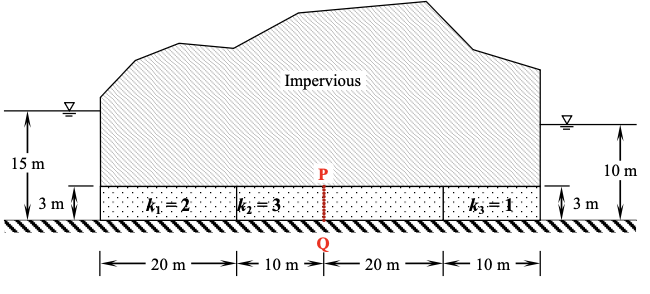
\includegraphics[width=0.6\columnwidth]{figs/Q56.png} 
    \caption{}
    \label{fig:placeholder}
\end{figure}

\begin{enumerate}
\begin{multicols}{4}
    \item $\frac{7}{12}$
    \item $\frac{1}{2}$
    \item $\frac{9}{16}$
    \item $\frac{3}{4}$
\end{multicols}
\end{enumerate}

\item A $4 \ m$ wide rectangular channel, having bed slope of $0.001$ carries a discharge of $16 \ \text{m}^3/\text{s}$. Considering Manning's roughness coefficient = $0.012$ and $g = 10 \ \text{m/s}^2$, the category of the channel slope is  \hfill \brak{GATE \ CE \ 2016}


\begin{enumerate}
    \item horizontal
    \item mild
    \item critical
    \item steep
\end{enumerate}

\item A sector gate is provided on a spillway. Assuming $g = 10 \ \text{m/s}^2$, the resultant force per meter length (expressed in kN/m) on the gate will be \_\_\_\_\_\_ \hfill \brak{GATE \ CE \ 2016}

\begin{figure}[H]
    \centering
    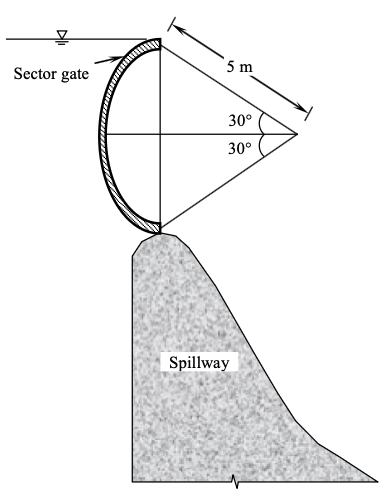
\includegraphics[width=0.6\columnwidth]{figs/Q58.png} 
    \caption{}
    \label{fig:placeholder}
\end{figure}

\item A hydraulically efficient trapezoidal channel section has a uniform flow depth of $2 \ m$. The bed width (expressed in m) of the channel is \_\_\_\_\_\_ \hfill \brak{GATE \ CE \ 2016}

\item Effluent from an industry 'A' has a pH of $4.2$. The effluent from another industry 'B' has double the hydroxyl (OH$^-$) ion concentration than the effluent from industry 'A'. pH of effluent from the industry 'B' will be \_\_\_\_\_\_ \hfill \brak{GATE \ CE \ 2016}

\item An electrostatic precipitator (ESP) with $5600 \ \text{m}^2$ of collector plate area is $96 \%$ efficient in treating $185 \ \text{m}^3/\text{s}$ of flue gas from a $200 \ \text{MW}$ thermal power plant. It was found that in order to achieve $97 \%$ percent efficiency, the collector plate area should be $6100 \ \text{m}^2$. In order to increase the efficiency to $99 \%$, the ESP collector plate area (expressed in $\text{m}^2$) would be \_\_\_\_\_\_ \hfill \brak{GATE \ CE \ 2016}

\item The 2-day and 4-day BOD values of a sewage sample are $100 \ \text{mg/L}$ and $155 \ \text{mg/L}$, respectively. The value of BOD rate constant (expressed in per day) is \_\_\_\_\_\_ \hfill \brak{GATE \ CE \ 2016}

\item A two lane, one-way road with radius of $50 \ m$ is predominantly carrying lorries with wheelbase of $5 \ m$. The speed of lorries is restricted to be between $60 \ \text{kmph}$ and $80 \ \text{kmph}$. The mechanical widening and psychological widening required at $60 \ \text{kmph}$ are designated as $w_{me,60}$ and $w_{ps,60}$, respectively. The mechanical widening and psychological widening required at $80 \ \text{kmph}$ are designated as $w_{me,80}$ and $w_{ps,80}$, respectively. The correct values of $w_{me,60}$, $w_{ps,60}$, $w_{me,80}$, $w_{ps,80}$ respectively are  \hfill \brak{GATE \ CE \ 2016}
\begin{enumerate}
    \item $0.89$ m, $0.50$ m, $1.19$ m, and $0.50$ m
    \item $0.50$ m, $0.89$ m, $0.50$ m, and $1.19$ m
    \item $0.50$ m, $1.19$ m, $0.50$ m, and $0.89$ m
    \item $1.19$ m, $0.50$ m, $0.89$ m, and $0.50$ m
\end{enumerate}

\item While traveling along and against the traffic stream, a moving observer measured the relative flows as $50 \ \text{vehicles/hr}$ and $200 \ \text{vehicles/hr}$, respectively. The average speeds of the moving observer while traveling along and against the stream are $20 \ \text{km/hr}$ and $30 \ \text{km/hr}$, respectively. The density of the traffic stream \brak{expressed \ in \ vehicles/km} is \_\_\_\_\_\_ \hfill \brak{GATE \ CE \ 2016}

\item The vertical angles subtended by the top of a tower $T$ at two instrument stations set up at $P$ and $Q$ are shown. The two stations are in line with the tower and spaced at a distance of $60 \ m$. Readings taken from these two stations on a leveling staff placed at the benchmark (BM = $450.000 \ m$) are also given. The reduced level of the top of the tower $T$ \brak{expressed \ in \ m} is \_\_\_\_\_\_ \hfill \brak{GATE \ CE \ 2016}

\begin{figure}[H]
    \centering
    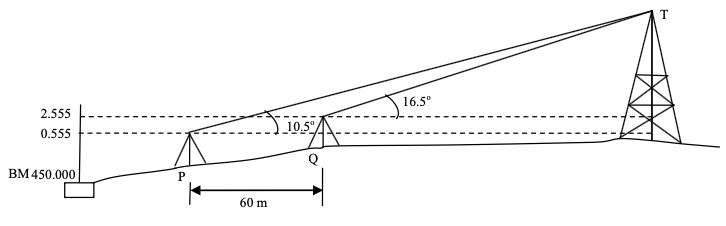
\includegraphics[width=0.6\columnwidth]{figs/Q65.png} 
    \caption{}
    \label{fig:placeholder}
\end{figure}


\end{enumerate}
\end{document}
